\newpage
\section{Setup and Simulation}
\begin{figure}[!h]
  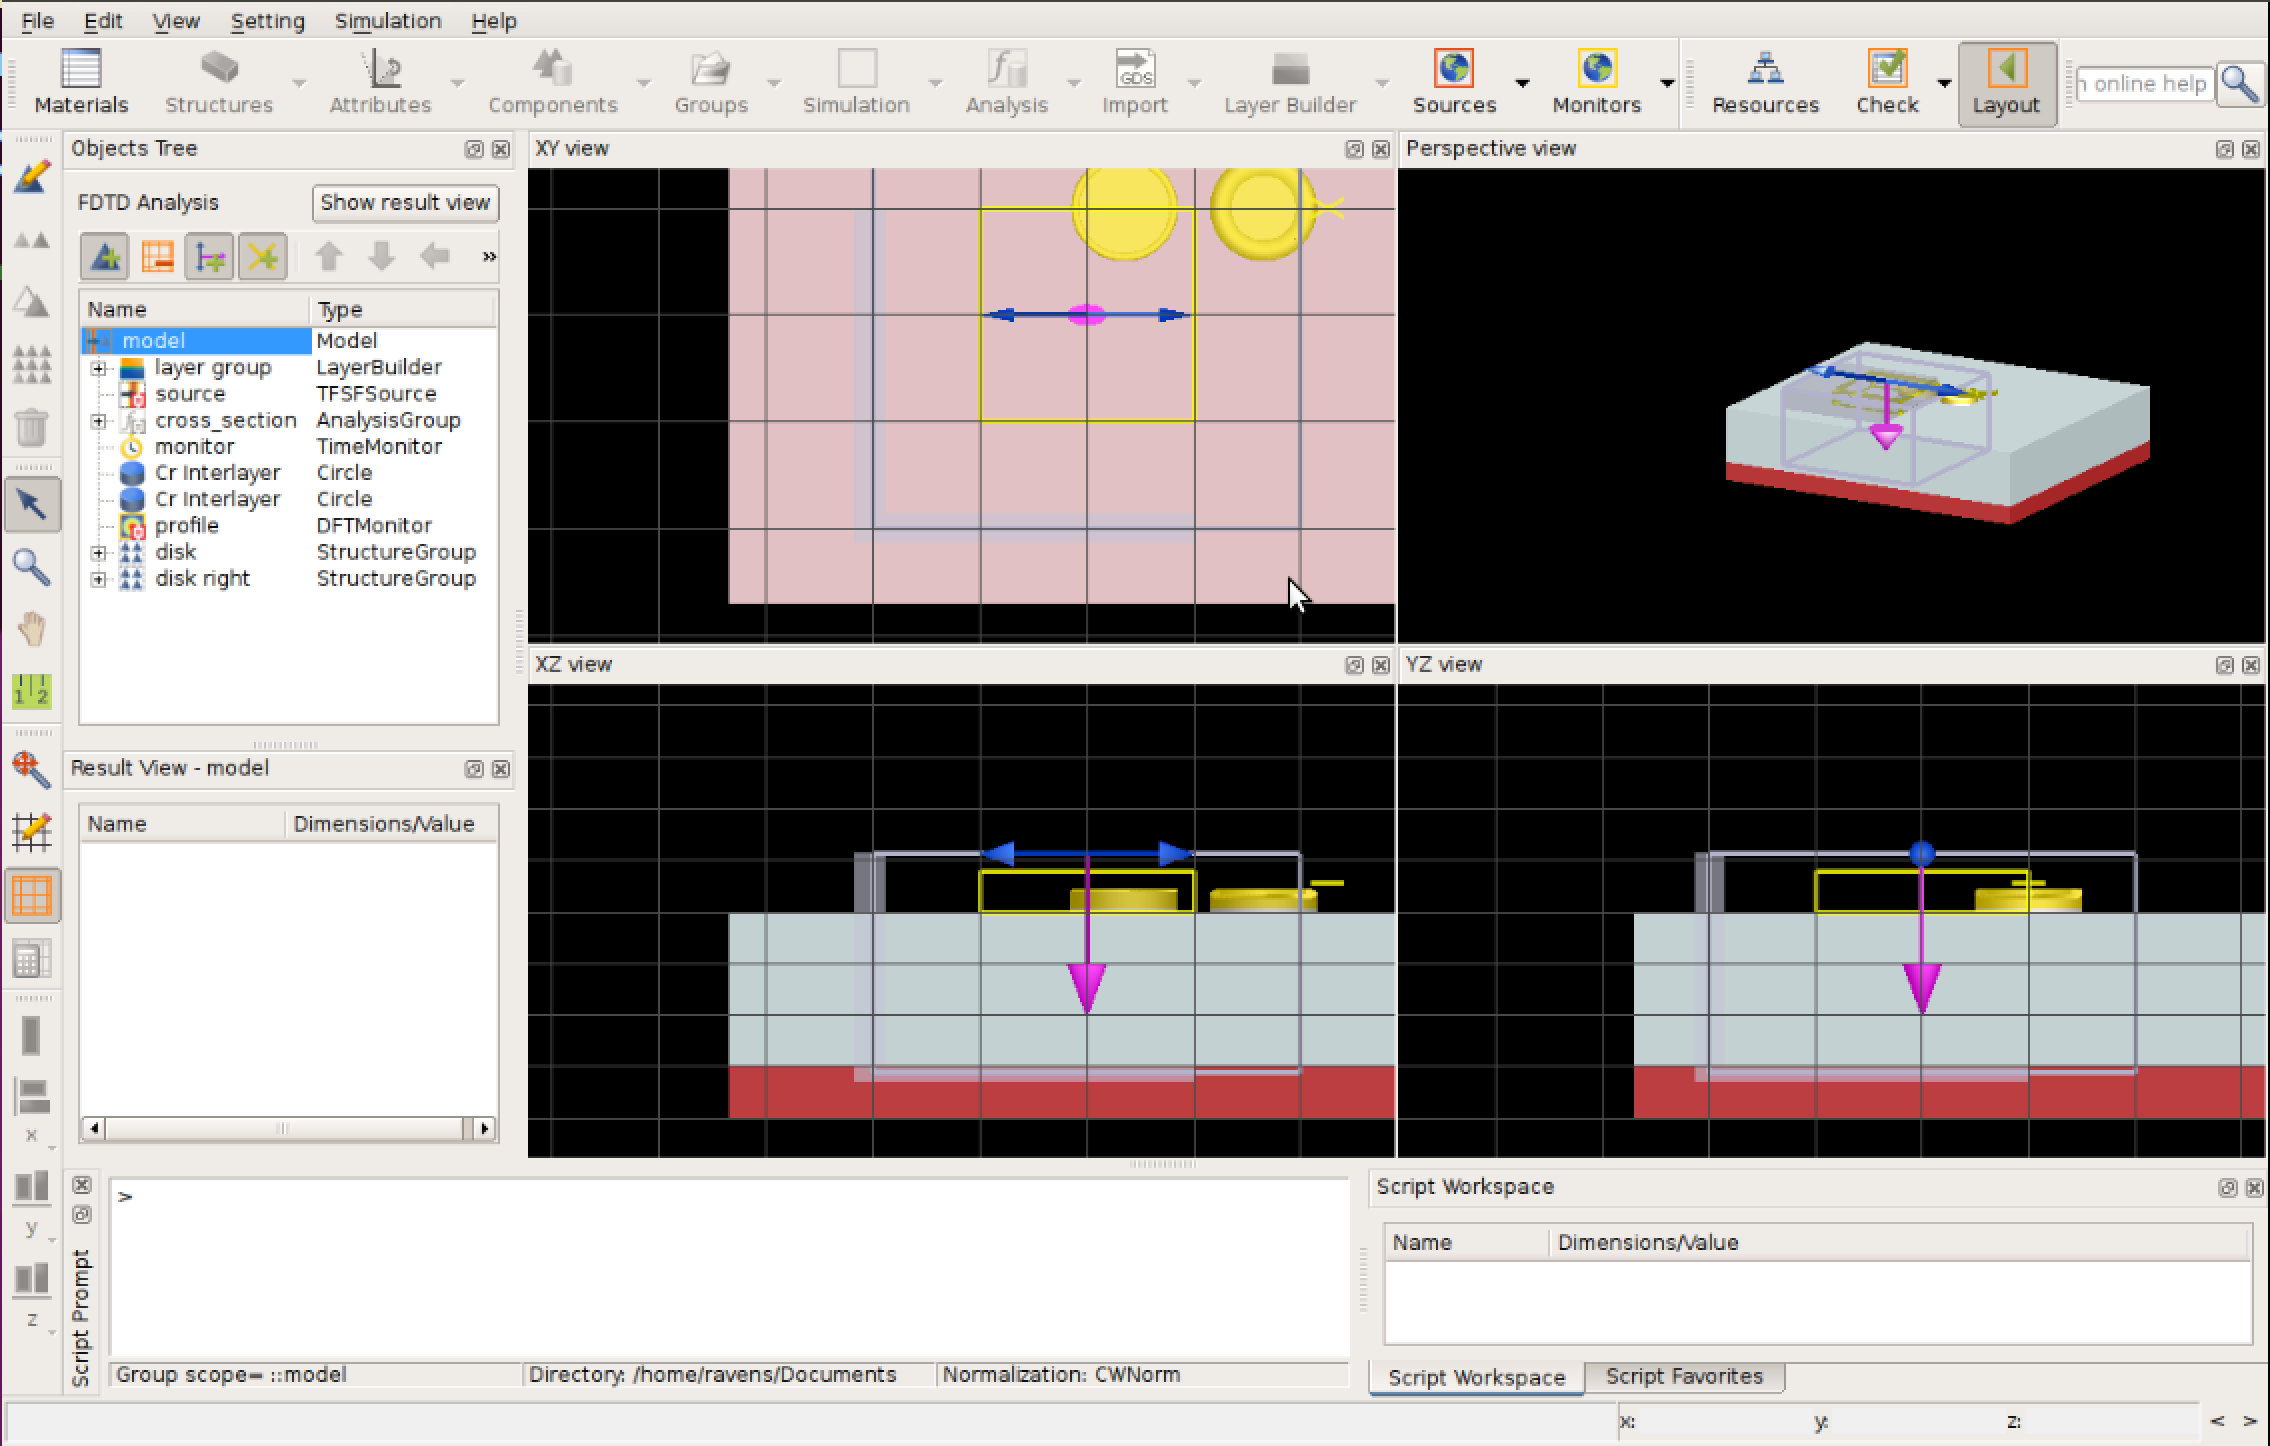
\includegraphics[width=\textwidth]{./images/lumerical.png}
  \caption{The experimental setup of \cite{heeg} simulated in lumerical FDTD. Two gold discs with a radius of \SI{50}{nm} are placed \SI{30}{nm} apart on SiO$_2$ on a \SI{5}{nm} Cr interlayer. The upper corners of the gold discs are rounded with a radius of \SI{2}{nm}. The simulation observes an area of $\SI{400}{nm}\times\SI{400}{nm}$ with a grid size of \SI{0.5}{nm}. To improve simulation time and memory consumption, only the lower left quarter is calculated and reproduced to the other quarters by using the mirror symmetry of the system.}
\end{figure}

\begin{figure}[!h]
  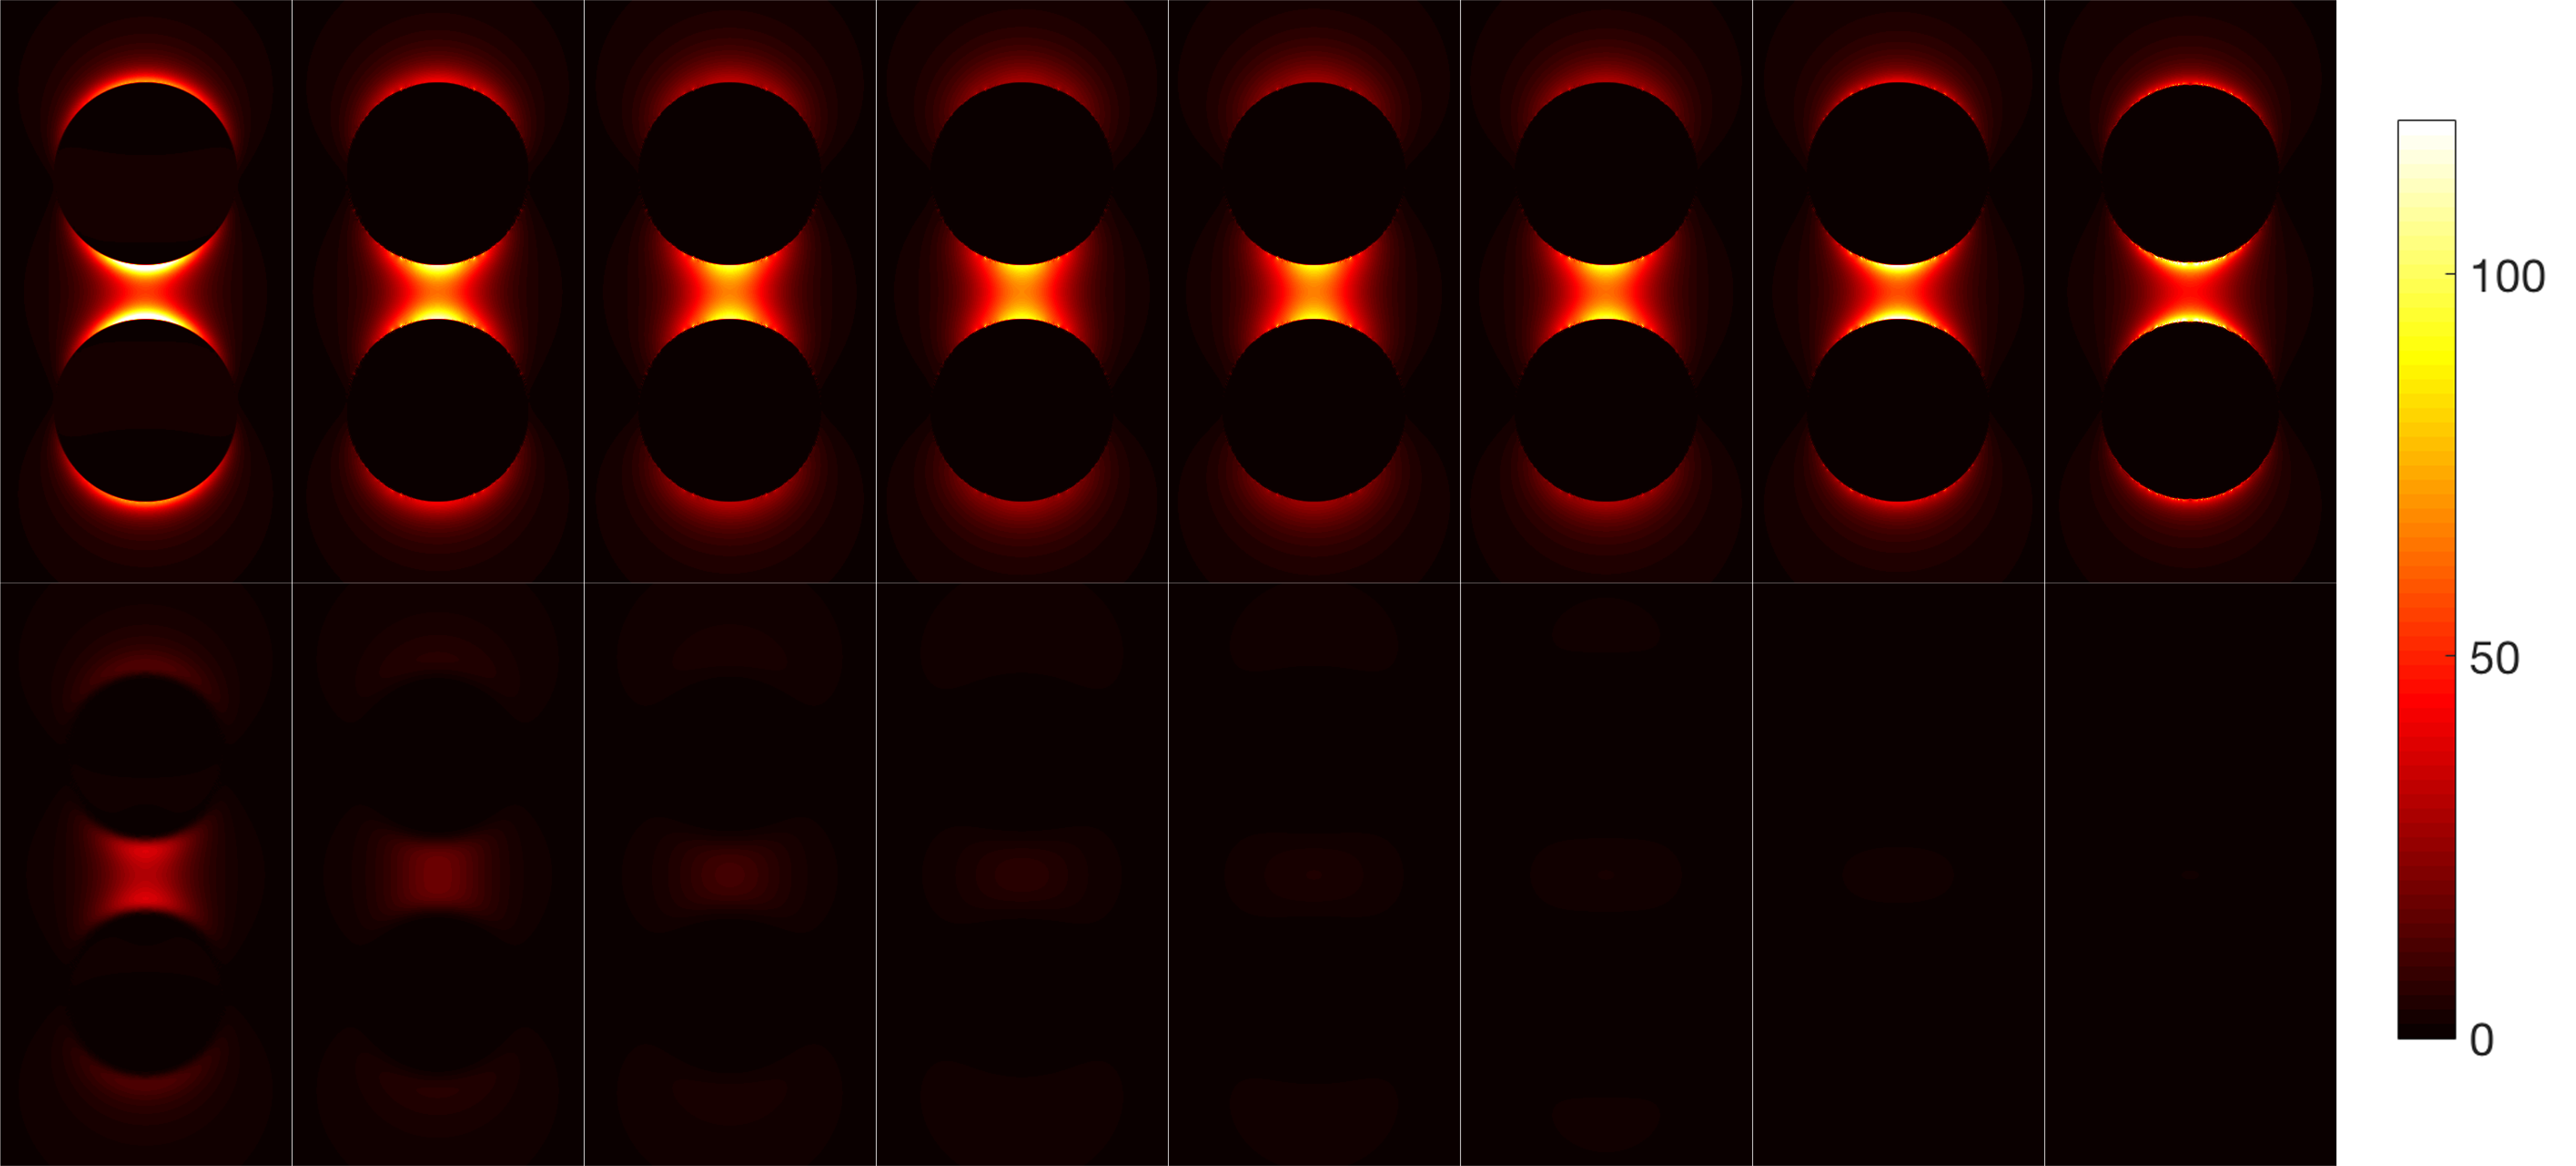
\includegraphics[width=\textwidth]{./images/simulation-slices.png}
  \caption{Slices of the simulation's result in the $x,y$-plane as near field enhancement $|E/E_0|^2$. Starting at the top left at $z=\SI{0}{nm}$ continuing in \SI{5}{nm} steps until $z=\SI{80}{nm}$.}
\end{figure}

\begin{figure}[!h]
  \centering
  \begin{subfigure}{0.50\textwidth}
    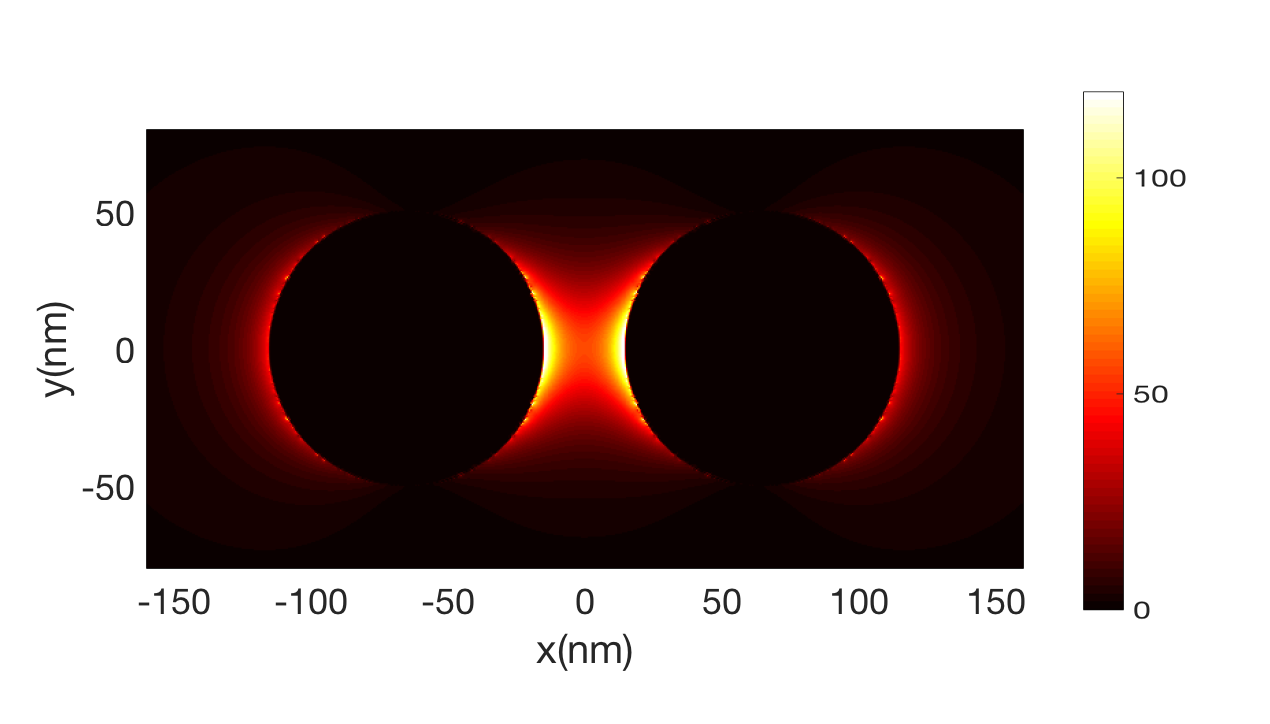
\includegraphics[width=\textwidth]{./images/40nm.png}
  \end{subfigure}
  ~
  \begin{subfigure}{0.40\textwidth}
    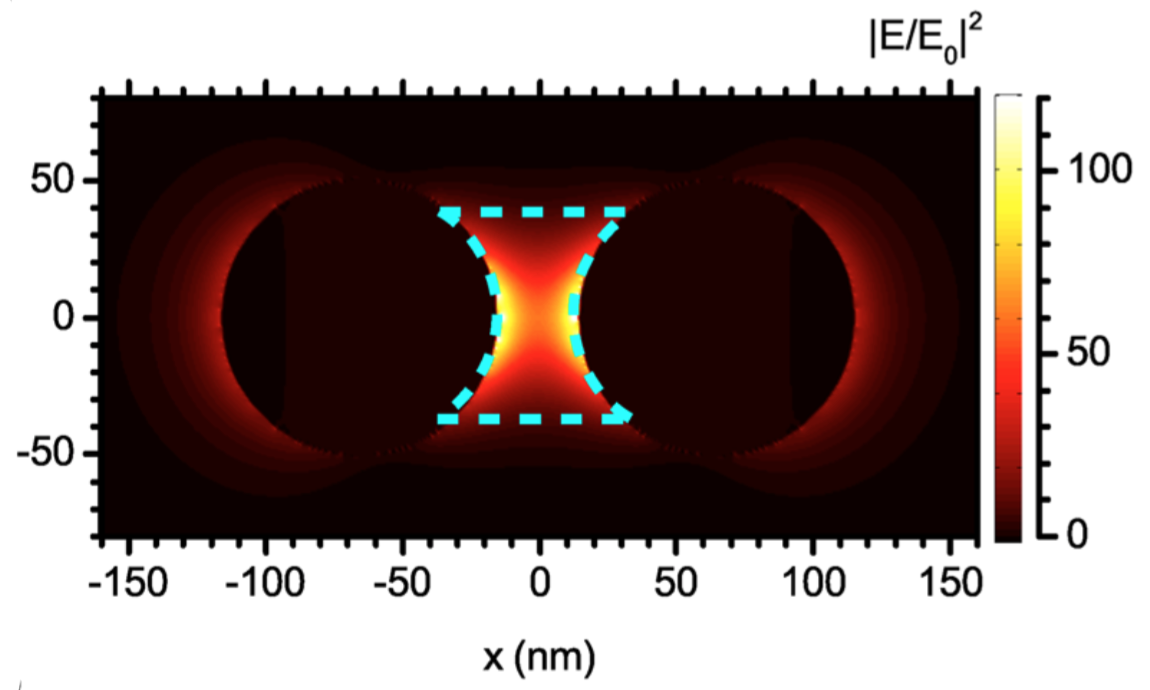
\includegraphics[width=\textwidth]{./images/local-enhancement-heeg.png}
  \end{subfigure}
  \caption{\textbf{(a)} Near field enhancement $|E/E_0|^2$ in the $x,y$-plane at $z=\SI{40}{nm}$. \textbf{(b)} Original results by \cite{heeg}.}
\end{figure}


\begin{figure}[!h]
  \centering
  \begin{subfigure}{0.45\textwidth}
    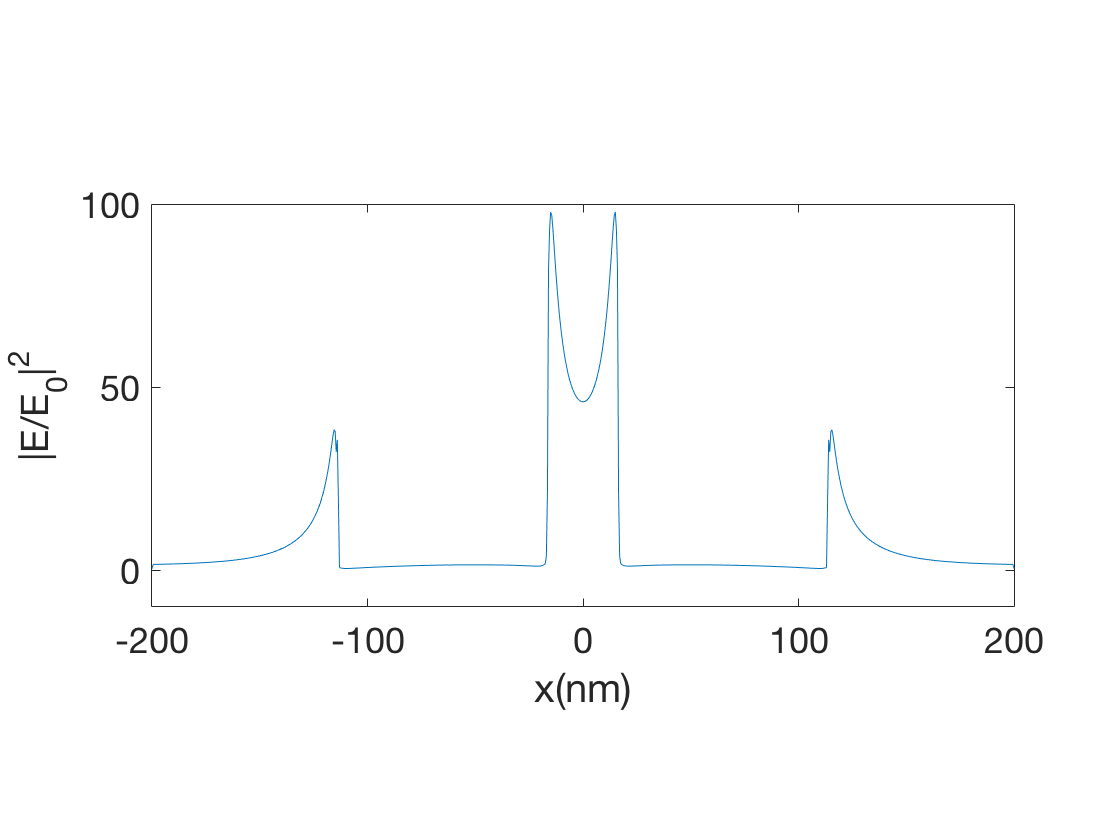
\includegraphics[width=\textwidth]{./images/40nm-y.png}
  \end{subfigure}
  ~
  \begin{subfigure}{0.45\textwidth}
    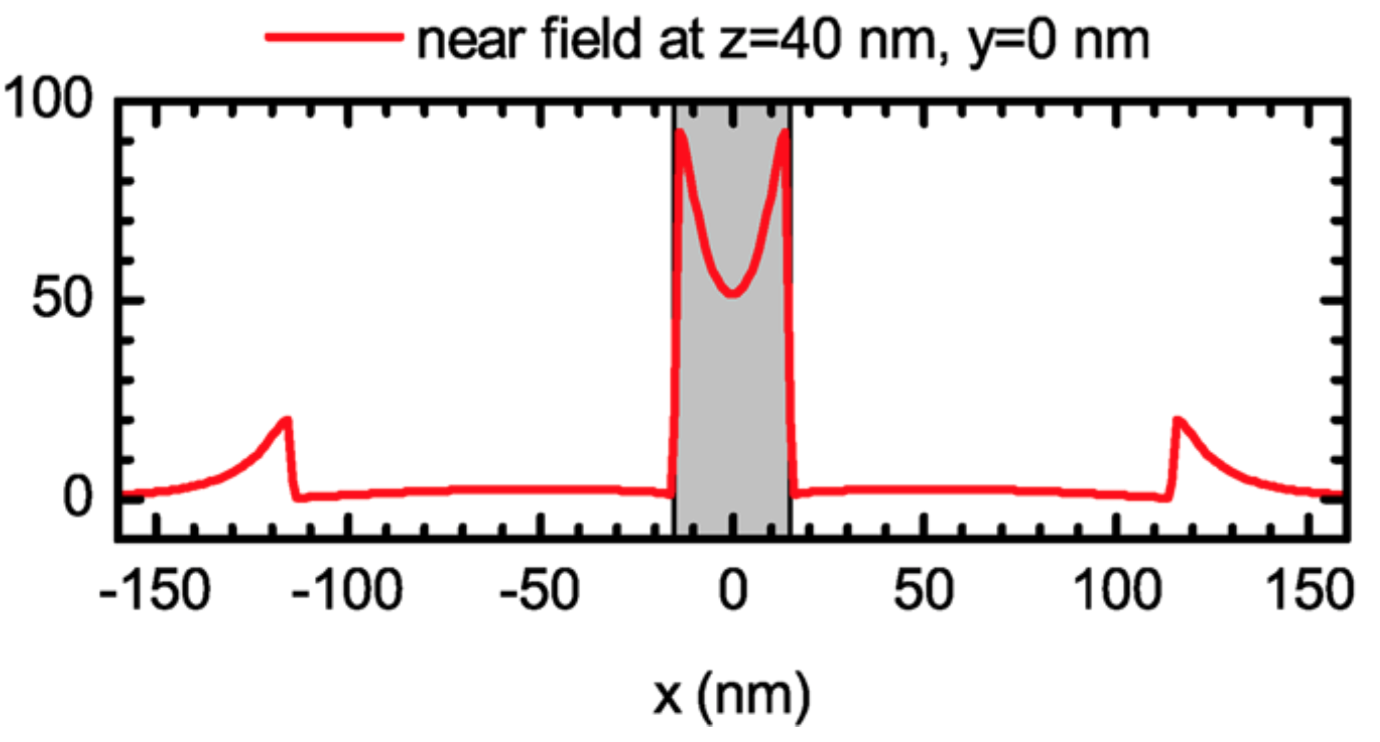
\includegraphics[width=\textwidth]{./images/heeg-y-line.png}
  \end{subfigure}
  \caption{\textbf{(a)} Near field enhancement $|E/E_0|^2$ in the $x,z$-plane at $y=0$. \textbf{(b)} Original results by \cite{heeg}.}
\end{figure}

\newpage
\null
